\documentclass[a4paper,12pt]{article}
\usepackage{amsthm}
\usepackage{amssymb}
\usepackage{indentfirst}
\usepackage{hyperref}
\hypersetup{
    colorlinks,
    linkcolor=black,
}
%\usepackage{tikz}
\usepackage{tkz-graph}
\usetikzlibrary{arrows}
\SetVertexNormal[	Shape		=	circle,
					FillColor	=	white,
					LineWidth	=	1pt,
					MinSize=0.3cm]
\SetUpEdge[lw			=	1.5pt,
			color		=	black,
			labelcolor	=	white,
			labeltext	=	red,
			labelstyle	=	{sloped,text=black}]
\usepackage{graphicx,subcaption}

%\newcounter{counter_methods}[subsection]

\theoremstyle{plain}
%\newtheorem{theorem}{Theorem}[section]
%\newtheorem{lemma}[theorem]{Lemma}
\newtheorem*{theorem}{Theorem}
\newtheorem*{lemma}{Lemma}
\newtheorem{claim}{Claim}
 
\theoremstyle{definition}
\newtheorem*{corollary}{Corollary}
\newtheorem{problem}{Exercise}[section]
\newtheorem*{definition}{Definition}
\newtheorem{method}{Method}[subsection]
\renewcommand{\themethod}{\arabic{method}}
\newtheorem{invariant}{Invariant}[subsection]
\renewcommand{\theinvariant}{\arabic{invariant}}
\newtheorem{assumption}{Assumption}[subsection]
\renewcommand{\theassumption}{\arabic{assumption}}
 
\theoremstyle{remark}
\newtheorem*{nonum}{Solution}
\newtheorem*{example}{Example}

\begin{document}

\tableofcontents





\newpage
\section{Algorithm design paradigms}
\textbf{Algorithm design:} no single "silver bullet" for solving problems.

\textbf{Some design paradigms:}
\begin{enumerate}
\item \textbf{divide and conquer} (merge sort as the canonical example)
\item \textbf{randomized algorithms} (coin flipping in quick sort with randomized pivot choosing, design of hash functions)
\item \textbf{greedy algorithms} (like Dijkstra shortest path)
\item \textbf{dynamic programming} (sequence alignment, distributed shortest path)
\end{enumerate}





\newpage
\section{Greedy algorithms}
\begin{definition}iteratively make "myopic" decisions, hope everything works out at the end\end{definition}



\subsection{Contrast with Divide \& Conquer}
\begin{itemize}
\item easy to propose multiple greedy algorithms for many problems
\item easy running time analysis (contrast with Master Method)
\item hard to establish correctness (contrast with staightforward inductive correctness proofs)
\end{itemize}

\textbf{[Danger]:} most greedy algorithms ara NOT correct (even if your intuition says otherwise)

\begin{example}Dijkstra shortest path algorithm for graphs with negative edge lengths is not correct\end{example}



\subsection{Proofs of correctness}
\begin{method}proof by induction ("greedy stays ahead")\end{method}
\begin{method}"exchange argument"\end{method}
\begin{method}whatever works!\end{method}



\subsection{Application: Optimal Caching}
\begin{itemize}
\item we have two ingredients: \textbf{small fast memory (cache)} and \textbf{big slow memory}
\item we processing sequence of \textbf{"page requests"}
\item on a \textbf{"fault" (cache miss)} we need to evict something from cache to make room -- \textbf{but what?}
\end{itemize}

We can have to sort of "page faults":
\begin{enumerate}
\item the one`s which we can`t do anything with (just because we can`t store all the memory in cache) -- they`re inevitable
\item the one`s that consequences of poor eviction choices
\end{enumerate}

\begin{theorem} [Belady, 1960] the \textbf{"furthest-in-future" algorithms} is optimal (i.e. minimizes the number of cache misses) [unimplementable] \end{theorem}

Why this unimplementable algorithm useful?
\begin{itemize}
\item serves as guideline for practical algorithms (e.g. least-recently-used, LRU should do well provided data exhibits locality of refence)
\item serves as idealized benchmark for caching algorithms
\end{itemize}

\begin{problem} find a simple proof for that theorem [tricky exchange argument]\end{problem}



\subsection{Scheduling application: problem definition and greedy algorithm}
\begin{itemize}
\item Setup: one shared resource (e.g., a processor) and many "jobs" to do (e.g., processes), assume there`re $n$ "jobs"
\item \textbf{[Question]:} in what order should we sequence the jobs?
\item \textbf{[Assume]:} each job $j$ has a weight $w_j \geq 0 $ ("priority") and length $l_j \geq	0$
\end{itemize}

\begin{definition}the completion time $c_j$ of job $j =$ sum of job lengths up to and including j \end{definition}

One natural \textbf{objective function} goal: minimize the weighted sum of completion times: $min \sum\limits_{i = 1}^{n}w_jC_j$

\begin{example}if all jobs have \textbf{same length`s} - we should schedule \textbf{larger-weight jobs earlier}\end{example}
\begin{example}if all jobs have \textbf{same weight`s} - we should schedule \textbf{shorter-length jobs earlier}\end{example}

\textbf{[Question]:} what if $w_i > w_j$ but $l_i > l_j$?

\textbf{[Idea]:} assign "scores" to jobs that are \textbf{increasing in weight} and \textbf{decreasing in length}, for example:
\begin{enumerate}
\item order jobs by decreasing value of $w_j - l_j$
\item order $w_j/l_j$
\end{enumerate}

We can find an example where two algorithms produce different outputs (at least one will be correct) like:
\begin{itemize}
\item first job: $l_1=5, w_1=3$
\item second job: $l_2=2, w_2=1$
\item sum of weighted completion times would be 23 and 22 respectively for difference and ratio ordering (\textbf{difference ordering is not optimal})
\item so \textbf{ratio ordering is not obvious correct} - needs proof of correctness
\end{itemize}



\subsection{Scheduling application: proof of correctness [$w_j/l_j$-ratio decreasing ordering]}

\begin{claim}Ordering jobs according to decreasing ratios $w_j/l_j$ is always correct\end{claim}

\textbf{[Assume]:} fix arbitrary input of n jobs (will proceed by contradiction).

\textbf{[Assume]:} let $\sigma =$ greedy schedule, $\sigma^* =$ optimal schedule.

\begin{proof}

\textit{[by an Exchange Argument]}

Plan - produce schedule even better than $\sigma^*$, contradicting purposted optimality of $\sigma^*$

[Assume]: all the ratios $w_j/l_j$ are distinct.

[Assume]: [just by renaming jobs] $\frac{w_1}{l_1} > \frac{w_2}{l_2} > \dots > \frac{w_n}{l_n}$.

Thus: greedy schedule $\sigma$ is just $1,2,3,\dots,n$

Thus: if optimal schedule $\sigma^* \neq \sigma$, then there are consecutive jobs $i, j$ with $i > j$ [only schedule where indices always go up is $1,2,3,\dots,n$]

\textbf{[Experiment]:} exchange order of i and j in $\sigma^*$ leaving other jobs unchanged

\begin{enumerate}
\item cost of exchange $= w_il_j$ [$C_i$ goes up by $l_j$]
\item benefit of exchange $= w_jl_i$ [$C_j$ goes down by $l_i$]
\end{enumerate}

\textbf{[Note]:} $i>j \Rightarrow \frac{w_i}{l_i} < \frac{w_j}{l_j} \Rightarrow w_il_j < w_jl_i \Rightarrow$ cost $<$ benefit

$\Rightarrow$ swap improves $\sigma^*$ that contradicts optimality of $\sigma^*$
\end{proof}



\subsection{Scheduling application: handling ties}

\begin{claim}Ordering jobs in nonincreasing order of ratio $w_j/l_j$ is always correct [even with ties]\end{claim}

\textbf{[Assume]:} fix arbitrary input of n jobs.

\textbf{[Assume]:} let $\sigma =$ greedy schedule, $\sigma^* =$ any other schedule.

\begin{proof}

Plan - will show $\sigma$ at least as good as $\sigma^* \Rightarrow$ implies that greedy schedule is optimal

[Assume]: [just by renaming jobs] $\frac{w_1}{l_1} \geq \frac{w_2}{l_2} \geq \dots \geq \frac{w_n}{l_n}$ [greedy schedule $\sigma$ is just $1,2,3,\dots,n$].

Consider arbitrary schedule $\sigma^*$. If $\sigma^* = \sigma \Rightarrow$ done.

Else recall $\exists$ consecutive jobs $i, j$ in $\sigma^*$ with $i > j$ 

\textbf{[Note]:} $i > j \Rightarrow \frac{w_i}{l_i} \leq \frac{w_j}{l_j} \Rightarrow w_il_j \leq w_jl_i \Rightarrow$ exchanging i and j in $\sigma^*$ has the benefit of $w_jl_i - w_il_j \geq 0$

\textbf{$\Rightarrow$ we don`t make $\sigma^*$ worse}. So, exchanging an "adjacent inversion" like $i, j$ only makes $\sigma^*$ better, and it decreases the number of inverted pairs

$\Rightarrow$ after at most $n \choose 2$ such exchanges, we can transform $\sigma^*$ into $\sigma$

$\Rightarrow \sigma$ at least as good as $\sigma^*$ 

$\Rightarrow$ greedy algorithm is optimal [proof is like applying BubbleSort()]
\end{proof}



\subsection{Minimum spanning trees (MST): problem definition}

\textbf{[Goal]:} connect a bunch of points together as cheaply as possible

\textbf{[Input]:} undirected graph G=(V,E) and a cost $c_e$ for each edge $e \in E$

[Assume]: adjacency list representation

[Assume]: OK if edge costs are negative

\textbf{[Output]:} minimum cost tree (sum of edge costs) $T \subseteq E$ that spans all vertices:
\begin{enumerate}
\item T has no cycles
\item the subgraph (V,T) is connected (contain path between each pair of vertices)
\end{enumerate}
We will set some non-important assumptions to get it easier (all the things will be correct without such assumptions):
\begin{assumption}input graph G is connected (else no spanning trees, easy to check in preprocessing, for example, with DFS)\end{assumption}
\begin{assumption}edge costs are distinct (still correct with ties, proof is more harder)\end{assumption}



\subsection{MST: Prim`s algorithm}
Example:\begin{figure}
\begin{subfigure}[b]{0.25\textwidth}
	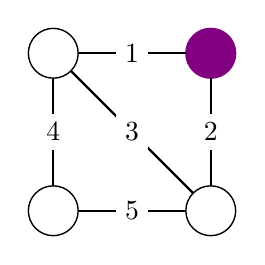
\begin{tikzpicture}[scale=0.5]
	\SetVertexNoLabel
		\Vertex[x=0 ,y=4]{A}
	\begin{scope}[VertexStyle/.append style = {color=violet}]
		\Vertex[x=4 ,y=4]{B}
	\end{scope}
		\Vertex[x=0 ,y=0]{C}
		\Vertex[x=4 ,y=0]{D}
	%	\tikzset{EdgeStyle/.append style = {bend left}}
		\Edge[label = $1$](A)(B)
		\Edge[label = $4$](A)(C)
		\Edge[label = $3$](A)(D)
		\Edge[label = $2$](B)(D)
		\Edge[label = $5$](C)(D)
	\end{tikzpicture}
\end{subfigure}
\begin{subfigure}[b]{0.25\textwidth}
	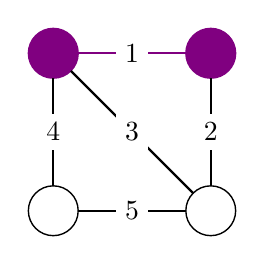
\begin{tikzpicture}[scale=0.5]
	\SetVertexNoLabel
	\begin{scope}[VertexStyle/.append style = {color=violet}]
		\Vertex[x=0 ,y=4]{A}
		\Vertex[x=4 ,y=4]{B}
	\end{scope}
		\Vertex[x=0 ,y=0]{C}
		\Vertex[x=4 ,y=0]{D}
	%	\tikzset{EdgeStyle/.append style = {bend left}}
		\Edge[label = $1$, color=violet](A)(B)
		\Edge[label = $4$](A)(C)
		\Edge[label = $3$](A)(D)
		\Edge[label = $2$](B)(D)
		\Edge[label = $5$](C)(D)
	\end{tikzpicture}
\end{subfigure}
\begin{subfigure}[b]{0.25\textwidth}
	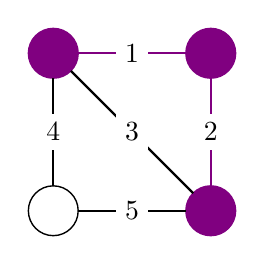
\begin{tikzpicture}[scale=0.5]
	\SetVertexNoLabel
	\begin{scope}[VertexStyle/.append style = {color=violet}]
		\Vertex[x=0 ,y=4]{A}
		\Vertex[x=4 ,y=4]{B}
	\end{scope}
		\Vertex[x=0 ,y=0]{C}
	\begin{scope}[VertexStyle/.append style = {color=violet}]
		\Vertex[x=4 ,y=0]{D}
	\end{scope}
	%	\tikzset{EdgeStyle/.append style = {bend left}}
		\Edge[label = $1$, color=violet](A)(B)
		\Edge[label = $4$](A)(C)
		\Edge[label = $3$](A)(D)
		\Edge[label = $2$, color=violet](B)(D)
		\Edge[label = $5$](C)(D)
	\end{tikzpicture}
\end{subfigure}
\begin{subfigure}[b]{0.20\textwidth}
	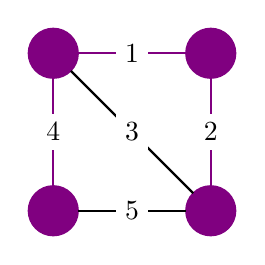
\begin{tikzpicture}[scale=0.5]
	\SetVertexNoLabel
	\begin{scope}[VertexStyle/.append style = {color=violet}]
		\Vertex[x=0 ,y=4]{A}
		\Vertex[x=4 ,y=4]{B}
		\Vertex[x=0 ,y=0]{C}
		\Vertex[x=4 ,y=0]{D}
	\end{scope}
	%	\tikzset{EdgeStyle/.append style = {bend left}}
		\Edge[label = $1$, color=violet](A)(B)
		\Edge[label = $4$, color=violet](A)(C)
		\Edge[label = $3$](A)(D)
		\Edge[label = $2$, color=violet](B)(D)
		\Edge[label = $5$](C)(D)
	\end{tikzpicture}
\end{subfigure}
\end{figure}

Prim`s MST Algorithm pseudo-code:
\begin{itemize}
\item initialize $X=[s]$, $s \in V$ chosen arbitrarily
\item $T =\varnothing$ [invariant: X = vertices spanned by tree-so-far T]
\item while $X \neq V$:
	\begin{itemize}
		\item let $e = (u,v)$ be the cheapest edge of G with $u \in X$, $v \notin X$ 
		\item add e to T
		\item add v to X
	\end{itemize}
	i.e., increasing $\#$ of spanned vertices in cheapest way possible
\end{itemize}



\subsection{MST: Prim`s algorithm correctness proof}
\begin{theorem}Prim`s algorithm always computes an MST. [by two claims]\end{theorem}

\begin{definition} a \underline{cut} of a graph $G=(V,E)$ is a partition of V into 2 non-empty sets (there`s $2^{n-1}$ possible cuts in graph)\end{definition} 

\begin{lemma}[\textbf{empty cut lemma}] a graph is \underline{not} connected $\iff \exists$ cut $(A,B)$ with no crossing edges\end{lemma}
\begin{proof}

\textbf{[$\Leftarrow$]:} assume the RHS. Pick any $u \in A$ and $v \in B$.

Since no edges cross (A,B), there is no u-v path in G $\Rightarrow$ G not connected

\textbf{[$\Rightarrow$]:} assume the LHS. Suppose G has no u-v path.

Define A = {vertices reachable from u in G} [u`s connected components].

Define B = {all other vertices}.

Note: no edges cross the cut (A,B), otherwise A would be bigger)
\end{proof}

\begin{lemma}[\textbf{double-crossing lemma}] suppose the cycle $C \subseteq E$ has an edge crossing the cut (A,B) then so does some other edge of C (at least twice, even number in general)\end{lemma}

\begin{corollary}[\textbf{lonely cut corollary}] if e is the only edge crossing some cut (A,B), then it is not in any cycle.\end{corollary}

\begin{claim} Prim`s algorithm outputs a spanning tree\end{claim}
\begin{proof}
\begin{enumerate}
	\item algorithm maintains invariant that T spans X [by straightforward induction]
	\item can`t get stuck with $X \neq V$ (otherwise the cut (X,V-X) must be empty, by Empty-cut lemma input graph G is disconnected)
	\item no cycles ever get created in T (by lonely cut corollary - we add edge, that first crosses X and V-X - no way to create cycle)
\end{enumerate}
\end{proof}

[MST is unique if edge costs are distinct]

\begin{claim}
Cut property: consider an edge $e$ of $G$. Suppose there is a cut $(A,B)$ such that $e$ is the cheapest edge of $G$ that crosses it. Then $e$ belongs to the MST of $G$.
\end{claim}
\begin{proof}
Will argue by contradiction using an exchange argument [like in scheduling application]

Suppose there is an edge $e$ that is the cheapest one crossing a cut $(A,B)$, yet $e$ is not in the MST $T^*$

\underline{idea:} exchange $e$ with another edge in $T^*$ to make it even cheaper (contradiction)

\underline{note:} since $T^*$ is connected, must contain an edge $f (\neq e)$ crossing (A,B) [by cut lemma]

idea: exchange $e$ and $f$ ($f \in T^*$) to get a spanning tree cheaper than $T^*$ (contradiction) - it may work and may not work, we should exchange correct edge\dots

\underline{hope:} can always find suitable edge $e^`$ so that exchange yields bona fide spanning tree of G

let C = cycle created by adding $e$ to $T^*$

\underline{by double-crossing lemma}: some other edge $e^`$ of C [with $e^` \neq e$ and $e^` \in T^*$] crosses (A,B)

\begin{example}: $T = T^* \cup {e} - {e^`}$ is also a spanning tree\end{example}

Since $c_e < c_{e^`}$, $T$ cheaper than purported MST $T^*$	, contradictioin
\end{proof}

\begin{claim} Cut property $\Rightarrow$ Prim`s algorithm is correct\end{claim}
\begin{proof}
Prim`s algorithm outputs a spanning tree $T^*$ (by previous claim)

\underline{Key point:} Every edge $e \in T^*$ is explicitly justified by the Cut property

$\Rightarrow T^*$ is a subset of the MST

$\Rightarrow$ since $T^*$ is already a spanning tree, it must be the MST
\end{proof}



\subsection{MST: Prim`s algorithm fast implementation}
\begin{itemize}
	\item $O(n)$ iterations
	\item $O(m)$ time per iteration
	\item \textbf{$\Rightarrow O(mn)$ time}
\end{itemize}

\begin{example}use heap to store edges, with keys $=$ edge costs. This leads to $O(m log n)$ implementation of Prim`s algorithm\end{example}

\begin{invariant}elements in heap $=$ vertices of $V-X$\end{invariant}
\begin{invariant}for $v \in V-X key[v] =$ cheapest edge $(u,v)$ with $v \in X$ (or $+\inf$ if no such edge exist)\end{invariant}

\begin{example}can initiate heap with $O(m+n log n) = O(m log n)$ preprocessing ($O(m)$ to compute keys, $O(n log n)$ for $n-1$ inserts, $m \geq n-1$ since G is connected)\end{example}

\underline{note}: given invariants Extract-min yields next vertex $v \notin V$ and edge $(u,v)$ crossing $(X,V-X)$ to add to X and T respectively

Might need to recompute some keys to maintain Invariant2 after each Extract-min, pseudocode:
\begin{itemize}
\item when $v$ added to $X$
\item for each edge $(v,w) \in E$
	\begin{itemize}
		\item if $w \in V-X$
		[the only vertices whose key might have dropped]
		\begin{itemize}
			\item delete $w$ from heap
			[subtle exercise - delete from heap]
			\item recompute $key[w]:= min[key[w],c_vw]$
			\item re-Insert $w$ into heap
		\end{itemize}
		[update key if needed]
	\end{itemize}
\end{itemize}

\begin{itemize}
	\item dominated by time required for heap operations
	\item $n-1$ Inserts during preprocessing
	\item $n-1$ Extract-mins (one per iteration of while loop)
	\item each edge $(v,w)$ triggers one Delete/Insert combo (when it`s first end point gets sucked into X)
	\item $\Rightarrow O(m)$ heap operations (since $m \geq n-1$ as G is connected)
	\item \textbf{$\Rightarrow O(m log n)$ time}
\end{itemize}

\end{document}